\documentclass{article}
\usepackage[utf8]{inputenc}
\usepackage{titling}
\usepackage{graphicx}
\usepackage{xcolor}
\usepackage[colorlinks=true,linkcolor=darkgray]{hyperref}
\usepackage[spanish]{babel}


\title{Práctica 3.2: Servidor DNS Maestro con chroot y apparmor}
\author{Cristina Díaz García}
\date{Noviembre 2018}

\renewcommand\maketitlehooka{\null\mbox{}\vfill}
\renewcommand\maketitlehookd{\vfill\null}


\begin{document}

\addcontentsline{toc}{section}{Índice general}

\begin{titlingpage}
\maketitle
\end{titlingpage}

\newpage

\tableofcontents

\newpage

\section{Modificación de \textit{/etc/default/bind9}}

\begin{center}
	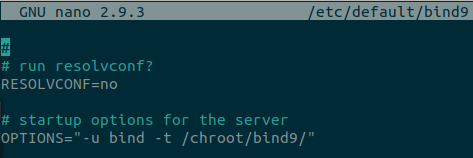
\includegraphics[scale=0.5]{Bind9.png} 
\end{center}

\section{Creación de directorios necesarios para bind9}

\begin{center}
	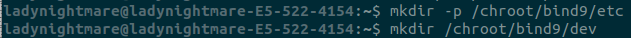
\includegraphics[scale=0.5]{mkdir1.png}
	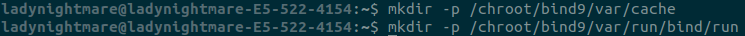
\includegraphics[scale=0.5]{mkdir2.png} 
\end{center}

\section{Movemos los ficheros de definición de zonas}

\begin{center}
	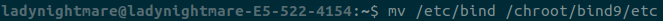
\includegraphics[scale=0.5]{mv1.png}
	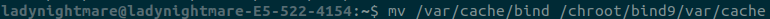
\includegraphics[scale=0.5]{mv2.png} 
\end{center}

\section{Creamos el enlace simbólico}

\begin{center}
	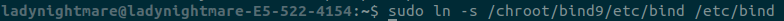
\includegraphics[scale=0.5]{link.png} 
\end{center}

\section{Creamos \textit{/dev/null} y \textit{/dev/random}}

\begin{center}
	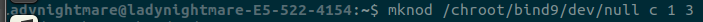
\includegraphics[scale=0.5]{mknod1.png} 
	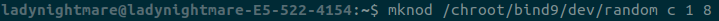
\includegraphics[scale=0.5]{mknod2.png} 
\end{center}

\section{Cambiamos el propietario}

\begin{center}
	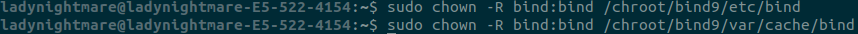
\includegraphics[scale=0.5]{chown.png} 
\end{center}

\section{Cambiamos los permisos}

\begin{center}
	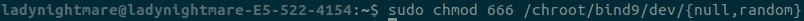
\includegraphics[scale=0.5]{chmod.png} 
\end{center}

\section{Editamos el archivo \textit{rsyslog}}

\begin{center}
	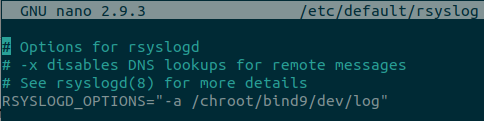
\includegraphics[scale=0.5]{rsyslog.png} 
\end{center}

\section{Iniciamos bind y comprobamos su estado}

\begin{center}
	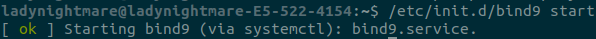
\includegraphics[scale=0.5]{startDemon.png}
	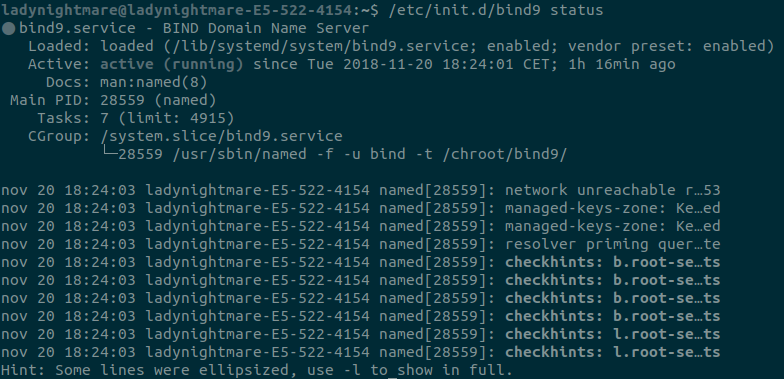
\includegraphics[scale=0.5]{statusDemon.png} 
\end{center}

\section{Comprobamos su funcionamiento}

\begin{center}
	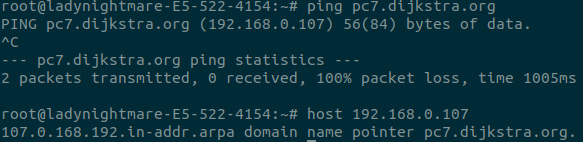
\includegraphics[scale=0.5]{hosts2.png} 
\end{center}

\end{document}
